\subsubsection{Mecanismos do NBTI}

% De acordo com \cite{Zeng} os mecanismos físicos do NBTI podem ser explicados através de três fenômenos não relacionados, que são: a geração de armadilhas na interface, o aprisionamento de lacunas e a geração de armadilhas no óxido do bulk.

O NBTI não pode ser explicado por um único mecanismo físico, mas por uma superposição de diversos processos \cite{Butzen}. Dois desses fenômenos são os mais aceitos, sendo eles: a geração de armadilhas na interface, o aprisionamento de lacunas.

O primeiro pode ser explicado pelo modelo de Reação-Difusão (RD), que diz que o NBTI é causado por ligações Si-H quebradas na interface entre o substrato e o oxido do gate. Essas ligações Si-H são formadas na fabricação do dispositivos para impedir que os átomos de silício fiquem com a valência incompleta após a colocação da camada de óxido de silício (SiO\small{2}) sobre o substrato. As ligações pendentes são denominadas estados de interface e podem voltar a ocorrer devido a campos elétricos elevados e alta temperatura \cite{Banaszeski}.

A Figura \ref{fig:PmosCrossSec} mostra as ligações Si-H na interface entre o gate e o substrato de um transistor PMOS.

\begin{figure}[H]
    \centering
    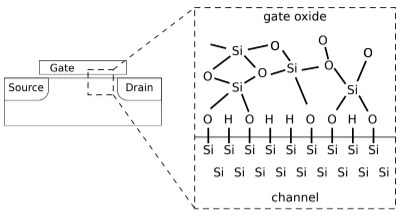
\includegraphics[scale=1]{figures/ReferencialTeorico/Cross section of a PMOS transistor.png}
    \caption{Seção da interface gate-substrato de um transistor PMOS. Fonte: \cite{Lorenz}}
    \label{fig:PmosCrossSec}
\end{figure}

Os estados de interface resultante deterioram parâmetros do transistor. Isso pode ser modelado pelo sistema RD, composto de dois processos: uma reação local e uma difusão dos produtos da reação.

A taxa de geração dessas interfaces é dada pela Equação \ref{eq:TaxaInteface} \cite{Lorenz}.

\begin{equation}
    \label{eq:TaxaInteface}
    \diff{N{\textsubscript it}}{t} = K{\scriptstyle F}(N{\scriptstyle 0} - N{\scriptstyle it}) - K{\scriptstyle R}N{\scriptstyle H}(0)N{\scriptstyle it}
\end{equation}

O primeiro termo do lado direito da equação mostra a componente de geração dos estados de interface, já o segundo termo descreve a regeneração das ligações, também denominada \textit{annealing} reverso, uma característica especial do NBTI.

$N\scriptstyle{0}$ representa a quantidade inicial de ligações Si-H, $N\scriptstyle{it}$ representa o número de estados de interface e $K\scriptstyle{R}$ é a taxa constante de criação de ligações quebradas. No termo de recuperação $N\scriptstyle{H}(0)$ representa o número de átomos de hidrogênio na interface do silício com o óxido, $K\scriptstyle{R}$ é a taxa constante de \textit{annealing} reverso das ligações incompletas e átomos de hidrogênio em ligações Si-H.

O lado direito da equação mostra que os estados de interface voltam a diminuir quando a condição de estresse é removida.

A criação de estados de interface é limitado pela difusão dos átomos de hidrogênio, como mostrado na Equação \ref{eq:TaxaDifusao}.

\begin{equation}
    \label{eq:TaxaDifusao}
    \diff{N{\scriptstyle it}}{t} = - D{\scriptstyle H}\diff{N{\scriptstyle H}}{x} + N{\scriptstyle H}\mu{\scriptstyle H}E{\scriptstyle ox}
\end{equation}

Onde $D\scriptstyle{H}$ representa o coeficiente de difusão, $\mu\scriptstyle{H}$ representa a mobilidade dos átomos de hidrogênio e $E\scriptstyle{ox}$ representa o campo elétrico que atravessa o óxido.

O segundo termo pode ser negligenciado para átomos ou moléculas eletricamente neutros \cite{Lorenz}. $K\scriptstyle{F}$, $K\scriptstyle{R}$ e $D\scriptstyle{H}$ dependem da temperatura. $K\scriptstyle{F}$ também depende do campo elétrico aplicado. Isso demonstra que as interfaces só são geradas quando um campo elétrico é aplicado, o que não é necessário para o \textit{annealing} e para a difusão.

As Equações \ref{eq:TaxaInteface} e \ref{eq:TaxaDifusao} formam um sistema que pode ser resolvido caso seja considerado que $N\scriptstyle{it}$ é muito menor que $N\scriptstyle{0}$. A Equação \ref{eq:ResultanteRD} mostra a solução desse sistema e a dependência da quantidade de interfaces com relação o tempo.

\begin{equation}
    \label{eq:ResultanteRD}
    N{\scriptstyle it} = \sqrt{\frac{K{\scriptstyle F}N{\scriptstyle 0}}{2K{\scriptstyle R}}}(D{\scriptstyle H}t)^{n}
\end{equation}

Onde n representa a constante exponencial de difusão e é sempre menor que 1, de forma que a geração das interfaces irá desacelerar com o tempo.

A variação Vth será proporcional ao $N\textsubscript{it}$, de forma que poderá ser escrito como mostrado na Equação \ref{eq:VthProp}, onde $\Phi\scriptstyle{S}$ é o potencial de superfície e $C{\scriptstyle ox}$ é a capacitância do óxido.

\begin{equation}
    \label{eq:VthProp}
    V{\scriptstyle th} \propto - \frac{qN{\scriptstyle it}(\Phi{\scriptstyle S})}{C{\scriptstyle ox}}
\end{equation}

Porém, esse fenômeno não explica completamente o fenômeno, não descrevendo corretamente a recuperação rápida que ocorre quando as condições de estresse não estão mais presentes \cite{Gilson}.

Um segundo mecanismo relacionado, denominado \textit{Trapping/Detrapping}, é baseado no aprisionamento de lacuna em defeitos no óxido pre-existentes ou provenientes de estresse elétrico \cite{Butzen}. O campo elétrico que gerado no gate quando o PMOS está negativamente polarizado causa o tunelamento de portadoras do canal nas falhas. Esse fenômeno vem sendo cada vez mais relevante na degradação por NBTI, considerando que falhas no óxido são mais comuns em transistores \textit{high-k}.

Cada armadilha apresenta tem como característica a probabilidade de capturar e liberar um portador e o valor do impacto na tensão de \textit{treshold} será gerado em caso de captura. As probabilidades tem relação com os tempos médios entre as capturas e emissões, já o impacto na tensão de \textit{treshold} tem relação com a localização em que a armadilha está localizada, podendo ser muito relevante caso obstrua o caminho de percolação do canal. 

% O modelo Trapping/Detrapping foi inicialmente desenvolvido para explicar a rápida recuperação do efeito de BTI. Assim surgiu um modelo misto, onde dois modelos coexistem: criação de defeitos na interface, dado pelo modelo Reaction-Difusion, e a captura e liberação de cargas por armadilhas pré-existentes no interior do óxido do transistor (HUARD, 2007). Neste modelo, a criação de defeitos na interface é o responsável pela parte permanente, não recuperável, da degradação enquanto as armadilhas, pré-existentes no interior do óxido, seriam responsáveis pela parte recuperável de BTI.

% Modelos mais recentes, (GRASSER, 2009) (KACZER, 2009), propõem que BTI pode ser explicado unicamente pelo efeito de captura e liberação de portadores no interior do dielétrico.

% No modelo Trapping/Detrapping, é explicada a variação de Vth pela pré-existência de armadilhas no interior do óxido, na qual cada armadilha tem como propriedades as probabilidades de captura e emissão, assim como, o desvio que causará no Vth. As probabilidades de captura e emissão são dadas pelo de tempo de captura e pelo tempo de emissão, que são os tempos médios transcorridos para que a armadilha capture um portador e emita esse portador, respectivamente. Esses tempos são log-uniformimente distribuídos, ou seja, armadilhas com diversas ordens de grandezas diferentes podem ser encontradas com a mesma probabilidade no óxido do transistor (GRASSER, 2010).

% De acordo com o modelo, quando uma armadilha é ocupada por um portador de carga (elétron ou lacuna) ela ficará eletricamente carregada. Assim, a tensão de limiar do transistor é alterada, de acordo com a localização da armadilha nas três dimensões do óxido (espessura, largura e comprimento). A localização na espessura do óxido determina o efeito eletrostático que a armadilha terá na porta e no canal de inversão do transistor, já a posição da armadilha na largura e no comprimento do óxido poderá determinar quão impactante será seu efeito na mobilidade dos portadores no transistor, já que o seu efeito eletrostático pode obstruir um caminho de percolação, ou percolation-path, no canal (KACZER, 2010) (Ver Seção 2.5), diminuindo drasticamente a sua condutividade. A localização da armadilha no comprimento do canal também determina o impacto da armadilha na tensão superficial ao longo da fonte e do dreno. Combinando todos os efeitos, dados pela localização da armadilha no canal, tem-se o desvio no Vth dado por uma determinada armadilha.

% Durante o período de estresse, armadilhas com diferentes tempos de captura e diferentes desvios de Vth são povoadas, alterando assim, a tensão limiar ao longo do tempo, conforme ilustrado na Figura 2.7, a seguir.


% Transistors with high-κ dielectric have higher density of pre-existing defects. From this point-of-view, hole trapping/detrapping is becoming the dominant contributor to NBTI degradation (KACZER, 2010).

Esses dois mecanismos podem sem considerados simultaneamente, sendo o primeiro responsável por uma componente permanente da degradação e o segundo responsável por uma componente recuperável da degradação \cite{Banaszeski}.

Cada um desses fenômenos contribui para a variação da tensão de treashold resultando na Equação \ref{eq:SomaVth}. Onde $V\scriptstyle{IT}$ á a contribuição das armadilhas na interface (primeiro mecanismo), $V\scriptstyle{HT}$ é a contribuição do aprisionamento em defeitos pré existentes e $V\scriptstyle{OT}$ é a contribuição do aprisionamento em defeitos gerados eletricamente (segundo mecanismo).

\begin{equation}
    \label{eq:SomaVth}
    \Delta V{\scriptstyle {th}} = \Delta V{\scriptstyle {IT}} + \Delta V{\scriptstyle {HT}} + \Delta V{\scriptstyle {OT}}
\end{equation}

A Equação \ref{eq:VthTempo} mostra uma aproximação da variação da tensão de treshold ao longo do tempo considerando um nó tecnológico específico e um certo conjunto de condições ambientais \cite{Butzen}.

\begin{equation}
    \label{eq:VthTempo}
    \Delta Vth = A(TSP.t)^n
\end{equation}

Onde A é uma constante que depende da tecnologia, t é o tempo, n é a constante exponencial do NBTI e TSP é a probabilidade do transistor estar negativamente polarizado.

O TSP de um transistor pode depender não só de seu duty cicle, mas também de sua posição na topologia do circuito. Por exemplo, no caso de dois transistores que compõe a malha de pull-up de uma porta NOR, o TSP do transistor superior depende apenas de seu sinal de entrada, já o TSP do inferior depende da combinação de seu sinal de entrada e do sinal de entrada do transistor superior, de forma que o transistor superior terá uma tendência maior a sofrer envelhecimento.

Quando não há campo elétrico atravessando o óxido do transistor, o que no caso dos PMOS ocorre quando a tensão de gate é positiva, há a recuperação das armadilhas de interface \cite{Chen}. Ou seja, em um circuito em que um transistor alterna entre fechado e aberto, haverá uma certa recuperação da degradação quando o transistor estiver fechado. A Figura \ref{fig:recover} exemplifica esse comportamento de estresse e relaxamento em um transistor.

\begin{figure}[H]
    \centering
    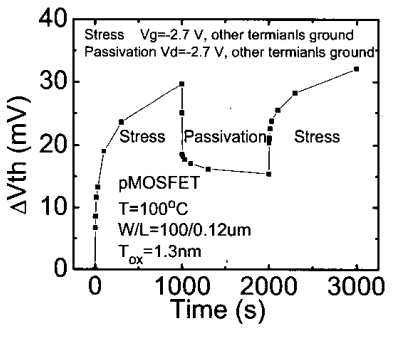
\includegraphics[scale=0.8]{figures/ReferencialTeorico/Recover.png}
    \caption{Estresse e relaxamento de um transistor. Fonte: \cite{Chen}}
    \label{fig:recover}
\end{figure}
